\documentclass[11pt, a4paper]{article}

% Styling lives in style/paper.sty
\usepackage{style/paper}

\title{A Test Paper for the Zig Build System}
\author{Research Group}
% The title-page date is derived from git by the build system (last commit
% touching this paper, or today when there are uncommitted changes). When
% gitdate.tex is absent (e.g. building directly with latexmk), fall back
% to \today.
\IfFileExists{gitdate.tex}{\input{gitdate.tex}}{\date{\today}}

\begin{document}

\maketitle

\begin{abstract}
	This paper exists to exercise the Zig-driven LaTeX build system. It imports a
	style file, pulls in section files, and contains floating environments so that
	the table of contents and list of figures require multiple render passes.
\end{abstract}

\tableofcontents
\listoffigures

\section{Introduction}
\label{sec:introduction}

This is the introduction of the test paper. Its purpose is to verify that
\verb|\input| of secondary files works from the Zig build system, and that the
table of contents picks up all sections across those files.

The remainder of the paper is organised as follows:
\cref{sec:method} describes the method,
\cref{sec:results} presents the results, and
\cref{sec:conclusion} concludes.

\subsection{Motivation}
\label{sec:motivation}

Most research groups build their papers with Makefiles or shell scripts. Using
Zig as the build system gives dependency tracking, caching, and a clean
separation between sources and build artifacts.

\subsection{Contributions}
\label{sec:contributions}

\begin{itemize}
  \item A test paper exercising all features needed by real papers.
  \item A Zig build graph that renders papers to PDF via \texttt{latexmk}.
  \item Automatic discovery of papers: drop a folder under \texttt{papers/}
        and a \texttt{zig build <name>} step appears.
\end{itemize}

\section{Method}
\label{sec:method}

This section contains mathematics and a table, exercising equation numbering
and the \texttt{booktabs} table style from \texttt{style/paper.sty}.

\subsection{Problem Statement}

Let $f \colon \mathbb{R}^n \to \mathbb{R}$ be the objective function. We seek
\begin{equation}
  \label{eq:objective}
  x^\ast = \arg\min_{x \in \mathbb{R}^n} f(x).
\end{equation}
The gradient of the objective in \cref{eq:objective} is denoted
$\nabla f(x)$, and the update rule is
\begin{equation}
  \label{eq:update}
  x_{k+1} = x_k - \alpha_k \nabla f(x_k),
\end{equation}
where $\alpha_k > 0$ is the step size at iteration $k$.

\subsection{Parameters}

\Cref{tab:parameters} lists the parameters used by the method described by
\cref{eq:update}.

\begin{table}[htbp]
  \centering
  \caption{Parameters of the optimisation method.}
  \label{tab:parameters}
  \begin{tabular}{llrl}
    \toprule
    \textbf{Parameter} & \textbf{Symbol} & \textbf{Value} & \textbf{Unit} \\
    \midrule
    Step size        & $\alpha$   & $0.01$ & --- \\
    Iterations       & $K$        & $1000$ & --- \\
    Tolerance        & $\varepsilon$ & $10^{-6}$ & --- \\
    Dimensionality   & $n$        & $64$   & --- \\
    \bottomrule
  \end{tabular}
\end{table}

\subsubsection{Step Size Schedule}
\label{sec:step-size}

The step size $\alpha_k$ decays geometrically\footnote{A geometric
schedule $\alpha_k = \alpha_0 \gamma^k$ with $\gamma \in (0, 1)$ is a
common baseline; more elaborate schemes such as Barzilai--Borwein
steps exist but are beyond the scope of this test paper.} rather than
being kept constant, which balances convergence speed against
oscillation near the optimum.

\section{Results}
\label{sec:results}

This section contains figures drawn with TikZ so that the paper needs no
binary image assets. Floating figures with captions populate the list of
figures and force the multi-pass rendering handled by \texttt{latexmk}.

\subsection{Convergence}

\Cref{fig:convergence} shows the convergence behaviour of the method from
\cref{sec:method}.

\begin{figure}[htbp]
  \centering
  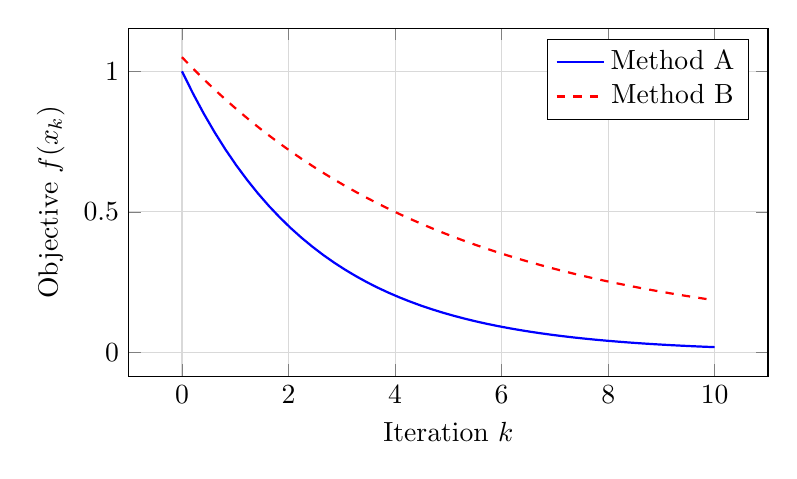
\begin{tikzpicture}
    \begin{axis}[
        width=0.8\textwidth,
        height=6cm,
        xlabel={Iteration $k$},
        ylabel={Objective $f(x_k)$},
        legend pos=north east,
        grid=both,
        grid style={gray!30},
      ]
      \addplot[blue, thick, domain=0:10, samples=50] {exp(-0.4*x)};
      \addlegendentry{Method A}
      \addplot[red, thick, dashed, domain=0:10, samples=50] {exp(-0.2*x) + 0.05};
      \addlegendentry{Method B}
    \end{axis}
  \end{tikzpicture}
  \caption{Convergence of the objective function for two methods.}
  \label{fig:convergence}
\end{figure}

\subsection{Architecture}

\Cref{fig:architecture} depicts the build pipeline that produced this
document.

\begin{figure}[htbp]
  \centering
  \begin{tikzpicture}[
      node distance=2.2cm,
      box/.style={rectangle, draw, rounded corners, minimum width=2.6cm,
                  minimum height=1cm, align=center, fill=blue!8},
      arrow/.style={-{Stealth}, thick},
    ]
    \node[box] (src) {Paper sources\\ \small \texttt{papers/<name>/}};
    \node[box, right=of src] (zig) {Zig build\\ \small \texttt{build.zig}};
    \node[box, right=of zig] (mk) {\texttt{latexmk}\\ \small multi-pass};
    \node[box, right=of mk] (pdf) {PDF\\ \small \texttt{zig-out/<name>.pdf}};
    \draw[arrow] (src) -- (zig);
    \draw[arrow] (zig) -- (mk);
    \draw[arrow] (mk) -- (pdf);
  \end{tikzpicture}
  \caption{The Zig build pipeline for a paper.}
  \label{fig:architecture}
\end{figure}


\section{Conclusion}
\label{sec:conclusion}

This paper demonstrated the full feature set the build system must support:
package imports, section imports, a table of contents, a list of figures,
cross-references (see \cref{sec:method}), and floating environments. If this
document renders, the multi-pass rendering performed by \texttt{latexmk} via
\texttt{zig build example-paper} is working correctly.

% Footnotes are collected here rather than at the page bottom
% (see style/paper.sty).
\clearpage
\theendnotes

\end{document}
